\documentclass[11pt,a4paper]{article}

\usepackage{../../templates/style}

\begin{document}

\begin{problem}{ท่อระบายน้ำ (Sewer)}{standard input}{standard output}{1 second}{16 megabytes}

เมืองแห่งหนึ่งมีพื้นที่เป็นรูปสี่เหลี่ยมขนาด $a$ แถวคูณ $b$ คอลัมน์และแบ่งเขตเป็นจำนวนเท่ากับ $a \times b$ เขต แต่ละเขตจะมีพิกัด $(i, j)$ โดยเขตที่พิกัด $(1, 1)$ จะอยู่ที่มุมซ้ายบนของพื้นที่สี่เหลี่ยม และแต่ละเขตจะมีท่อระบายน้ำเชื่อมต่อกับเขตเพื่อนบ้านหรือไม่ก็ได้ ดังแสดงในรูป (ให้เครื่องหมาย \textit{$\Leftrightarrow$ ลูกศร} แสดงถึงท่อระบายน้ำที่เชื่อมระหว่างเขต)


กำหนดให้เขตที่พิกัด $(1, 1)$ เป็นจุดเริ่มปล่อยน้ำทิ้ง โดยจะสามารถระบายน้ำทิ้งไปยังท่อระบายน้ำที่เชื่อมอยู่กับเขตนั้น ๆ และแต่ละท่อใช้เวลาระบายน้ำทิ้งจากเขตหนึ่งไปยังเขตหนึ่งด้วยเวลาหนึ่งหน่วย น้ำสามารถไหลได้ $4$ ทิศทาง คือไหลไปยังเขตทิศเหนือ ไหลลงเขตทิศใต้ ไหลไปเขตทางตะวันออก และ ไหลไปเขตทางตะวันตก โดยเขตรับน้ำจะไม่สามารถระบายน้ำกลับไปยังเขตก่อนหน้าที่ระบายน้ำมาให้

\begin{figure}[!h]
\centering
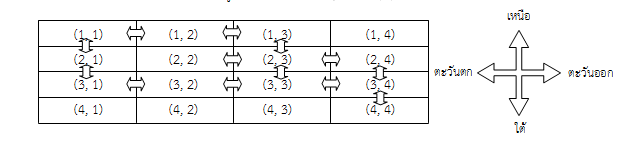
\includegraphics[width=1\textwidth]{../latex/img/1161/1161-1.png}
\end{figure}


โดยจากรูปตัวอย่างข้างบนนี้ น้ำทิ้งจะเริ่มต้นที่ $(1, 1)$ ในช่วงเวลาที่ $1$ และเคลื่อนไปสู่ $(2, 1)$ และ $(1, 2)$ ในช่วงเวลาที่ $2$ จากนั้นจึงไปสู่ $(3, 1)$ และ $(1, 3)$ ในช่วงเวลาที่ $3$ และถึง $(3, 2)$ กับ $(2, 3)$ ในช่วงเวลาที่ $4$ และสุดท้ายจึงมาบรรจบกันที่พิกัด $(3, 3)$ ในช่วงเวลาที่ $5$ ตามลำดับ

กำหนดให้แต่ละเขตสามารถมีรูปแบบการติดตั้งท่อระบายน้ำได้ทั้งหมด $4$ รูปแบบ เมื่อพิจารณาการเชื่อมต่อทางทิศตะวันออกและทิศใต้เท่านั้น ได้แก่ $R$ หมายถึงเขตนั้นมีท่อระบายน้ำเชื่อมกับเขตทิศตะวันออก, $D$ หมายถึงเขตนั้นมีท่อระบายน้ำเชื่อมกับเขตทิศใต้, $B$ หมายถึงเขตนั้นมีท่อระบายน้ำเชื่อมกับทั้งเขตทิศตะวันออกและทิศใต้, และ $N$ หมายถึงเขตนั้นไม่มีท่อระบายน้ำเชื่อมกับเขตทิศตะวันออกและทิศใต้

\bigskip
\underline{\textbf{โจทย์}}  จงเขียนโปรแกรมเพื่อคำนวณหาระยะเวลาที่น้อยที่สุด ที่น้ำทิ้งอย่างน้อย $2$ สายจะมาบรรจบกัน พร้อมทั้งบอกพิกัดของเขตที่น้ำทิ้งมาบรรจบกัน (รับประกันว่าข้อมูลนำเข้าทุกชุด จะมีเขตที่น้ำสองสายมาบรรจบกันที่เกิดขึ้นเร็วที่สุด เพียงเขตเดียวเสมอ) 


\InputFile

\textbf{บรรทัดแรก} รับค่าของตัวแปร $a$ และ $b$ โดยที่ $2 \leq a,b \leq 100$
\newpage

\textbf{บรรทัดที่ $2$ ถึง $a + 1$} แต่ละบรรทัดมีตัวอักษรทั้งหมด $b$ ตัว คั่นด้วยช่องว่าง แต่ละตัวระบุถึงสถานะการมีท่อระบายน้ำของเขตแต่ละเขตในพิกัด $(i, j)$ โดยเริ่มจากพิกัดที่ $(1, 1)$ ไปเรื่อยๆ ตามลำดับ และ $1 \leq i \leq a; 1 \leq j \leq b$


\OutputFile

\textbf{บรรทัดแรก} แสดงจำนวนเต็ม $1$ ตัว แสดงถึงช่วงเวลาที่น้ำทิ้งมาบรรจบกัน

\textbf{บรรทัดที่สอง} แสดงจำนวนเต็ม $2$ ตัว คั่นด้วยช่องว่าง ซึ่งเป็นพิกัด $(i, j)$ ที่น้ำทิ้งมาบรรจบกัน

\Examples

\begin{example}
\exmp{4 4
B R D N
D R B D
R R R D
N N N N}{5
3 3}%
\exmp{3 4
B B B D
D N R B
R R R N}{5
2 4}%
\end{example}


\Source

การแข่งขันคอมพิวเตอร์โอลิมปิกระดับชาติครั้งที่ 7 (NUTOI7)

\end{problem}

\end{document}